\section{Integração com middleware \textit{UbiquitOS}}

	Com intuito de exemplificar a utilização do \textit{UserDriver} e testar a integração do Sistema TRUE com o middleware \textit{UbiquitOS} foi desenvolvido uma aplicação para o middleware chamada \textit{UserApp} cujo diagrama de classe é mostrado na Figura~\ref{fig:diagrama-userapp}. Esta aplicação registra um \textit{listener} para ``escutar'' os eventos do \textit{UserDriver} chamado \textit{UserListener}. A Figura~\ref{fig:diagrama-userlistener} mostra o diagrama de classe do \textit{UserListener}.

		\begin{figure}[hbt]
			\begin{center}
				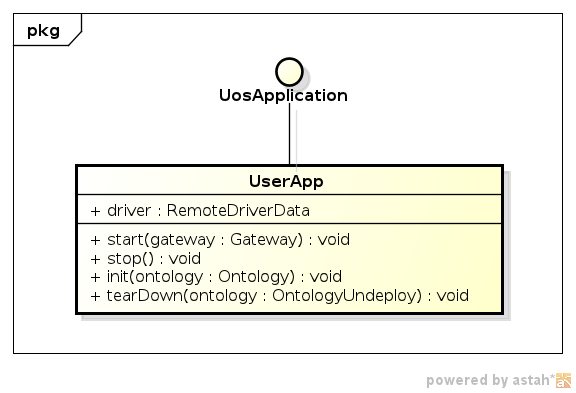
\includegraphics[scale=0.6]{figuras/5.Testes/diagrama-classe-user-ap.png}
			\end{center}
			\caption{Diagrama de Classe da aplicação \textit{UserApp}.}
			\label{fig:diagrama-userapp}
		\end{figure}

		\begin{figure}[hbt]
			\begin{center}
				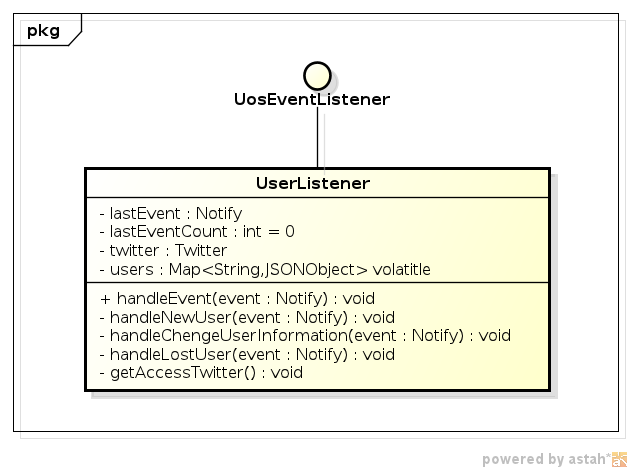
\includegraphics[scale=0.6]{figuras/5.Testes/diagrama-classe-user-listener.png}
			\end{center}
			\caption{Diagrama de Classe do \textit{listener} \textit{UserListener}.}
			\label{fig:diagrama-userlistener}
		\end{figure}

	Basicamente, quando o \textit{UserListener} obtém os eventos do \textit{UserDriver} envia mensagens pelo Twitter para os usuários no ambiente, conforme o evento recebido. A Figura~\ref{fig:diagrama-tweet} mostra o fluxo básico de execução do \textit{listener} e as mensagens padrões para cada tipo de evento recebido. Para enviar as mensagens pelo Twitter foi utilizado a biblioteca \textit{twitter4j}. 

	\begin{figure}[hbt]
			\begin{center}
				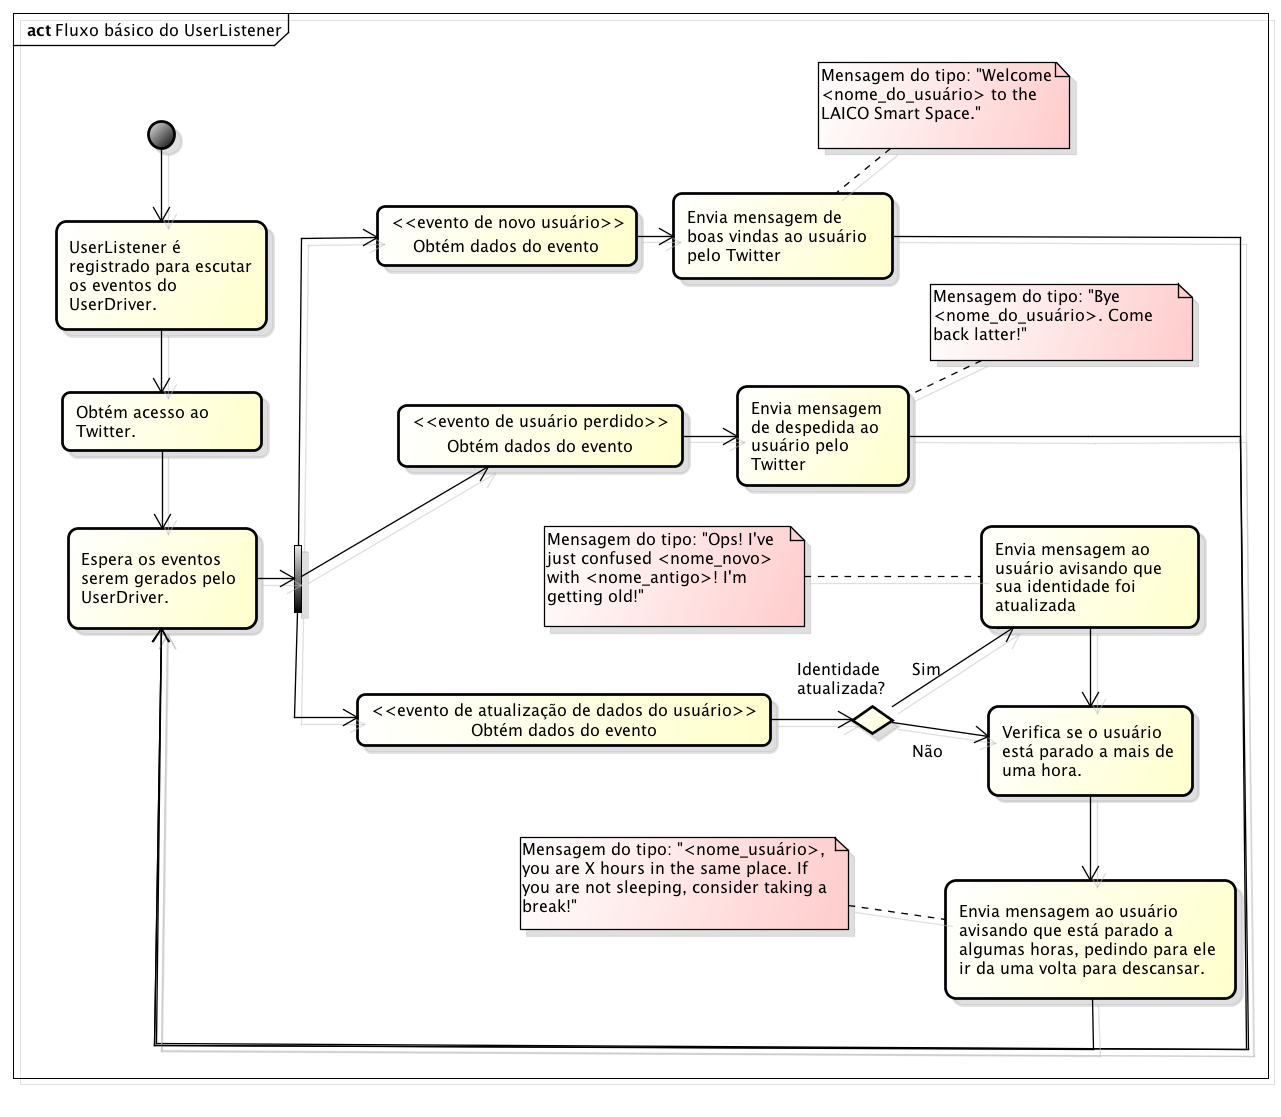
\includegraphics[scale=0.45]{figuras/5.Testes/diagrama-user-tweet.png}
			\end{center}
			\caption{Fluxo básico de execução do \textit{listener} \textit{UserListener}.}
			\label{fig:diagrama-tweet}
		\end{figure}

	Testes funcionais foram feitos com a aplicação mostrando que o driver consegue obter os dados íntegros do Sistema TRUE e gerar os eventos de maneira quase instantânea. Algumas vezes as mensagens demoravam a chegar ao Twitter, geralmente nos horários de ``pico'' quando o Twitter operava além da sua capacidade. A Figura~\ref{fig:tweets} mostra as mensagens geradas pela aplicação em um teste funcional, onde Danilo, um usuário cadastrado, entra no ambiente senta em uma mesa com seu notebook permanecendo no mesmo lugar por mais de uma hora, e logo depois deixa o ambiente.

	\begin{figure}[hbt]
			\begin{center}
				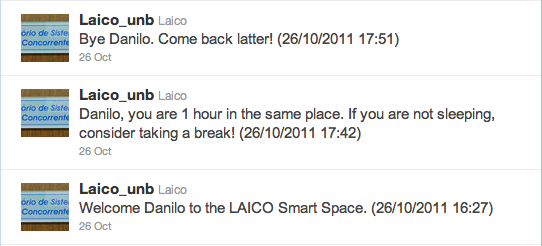
\includegraphics[scale=0.6]{figuras/5.Testes/tweets.png}
			\end{center}
			\caption{Exemplo das mensagens enviadas pelo Twitter aos usuários no ambiente.}
			\label{fig:tweets}
		\end{figure}	